% coding:utf-8

% Ausführen in R: 
% Sweave("C:/Daten/Daniel/studium/git_repo/sem2/stoc/sw08/sw08_1.Rnw",encoding='UTF-8')

\section{Aufgabe 1}

\subsection{a}
\[ F_x(x) = 1 - e^{-\lamda x} = u \]
\[ 1 - u = e^{-\lamda x} \]
\[ \ln(1-u) = -\lamda x \]
\[ x = -\frac{\ln(1-u)}{\lamda} = \triangleq F_x^{-1}(u) \]
\begin{Schunk}
\begin{Sinput}
> anz <- 1000
> x <- -(log(1-runif(n=anz,min=0,max=1)))/(2)
> hist(x)
\end{Sinput}
\end{Schunk}
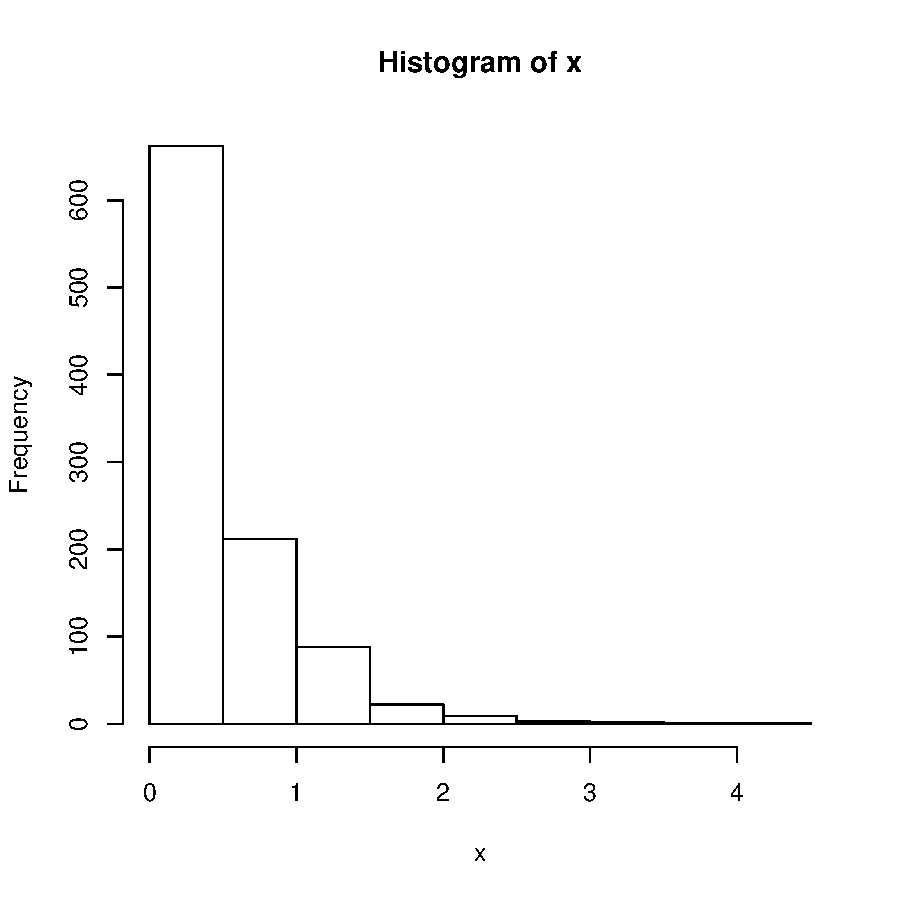
\includegraphics{sw08_1-001}

\subsection{b}
\begin{Schunk}
\begin{Sinput}
> anz <- 10000
> quantexp <- qexp((seq(1,anz,by=1)-0.5)/anz,rate=2)
> x <- -(log(1-runif(n=anz,min=0,max=1)))/(2)
> qx <- sort(x)
> plot(quantexp,qx)
\end{Sinput}
\end{Schunk}
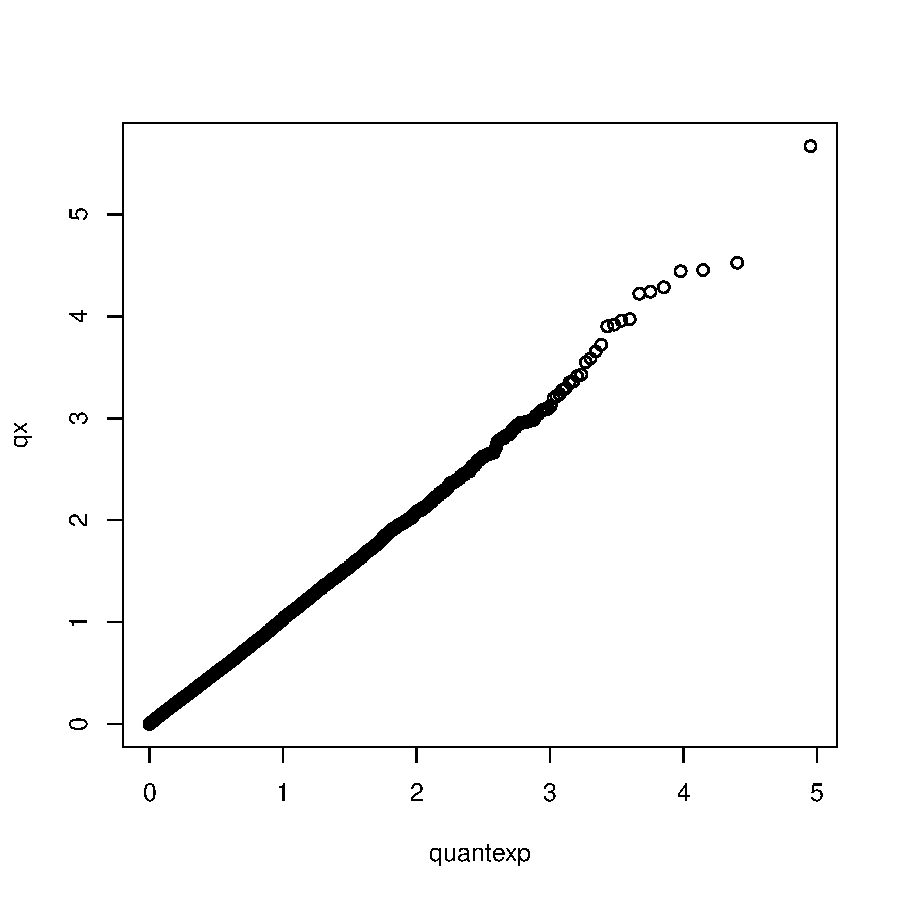
\includegraphics{sw08_1-002}
